\documentclass[main]{subfiles}


\title[AutoML: NAS]{Neural Architecture Search}
\subtitle{Speed-Up Techniques for Performance Estimation}
\author[Jovita Lukasik]{Jovita Lukasik}
\date{}

\titlebackground*{images/AutoML_NAS}

%\institute{}
%\date{}

\begin{document}
	
	\maketitle

%----------------------------------------------------------------------
\begin{frame}{Motivation}
\begin{itemize}
    \item Even with surrogate predictors, evaluating architectures involves \alert{at least partial training} — still slow at scale
    \item Two families of techniques avoid this bottleneck:
    \begin{itemize}
        \item \textbf{Learning curve extrapolation}: predict final accuracy from early training dynamics
        \item \textbf{Zero-cost proxies}: score of an \emph{untrained} network using at most a single forward and backward pass
    \end{itemize}
    \item Predictors can also be \alert{embedded into the search loop} to guide which candidates get evaluated next
\end{itemize}
\pause
\vspace{0.5em}
\begin{colorblock}[black]{sintefgrey}{Key Question}
How can we reduce the cost of NAS to \textbf{minutes instead of days} while still reliably identifying high-performing architectures?
\end{colorblock}
\vspace{0.5em}
% $\rightsquigarrow$ This video covers low-fidelity speed-up techniques and how predictors are embedded into search
\end{frame}
%----------------------------------------------------------------------

\begin{frame}{Overview of Speed-Up Techniques}
\begin{center}
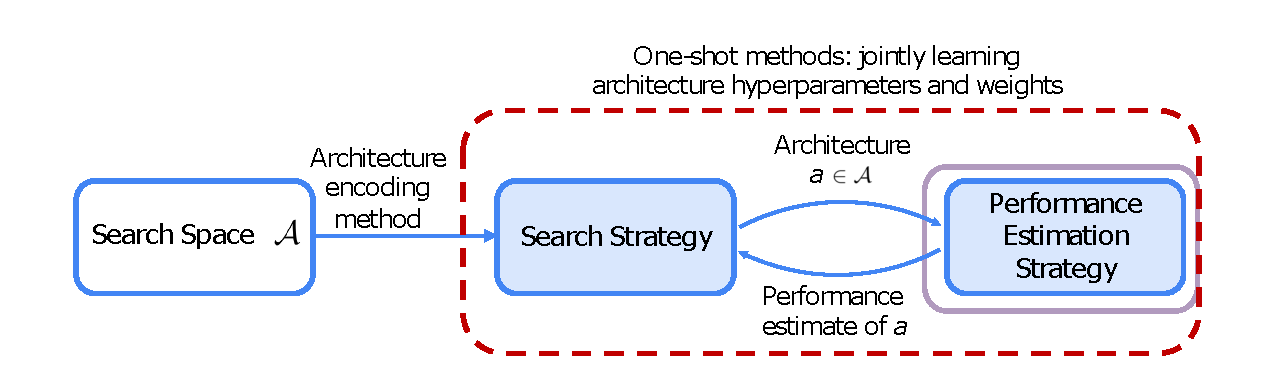
\includegraphics[height=3cm]{images/04/white_2023_nas_overview_3.pdf}
\captionof{figure}{Overview of neural architecture search ~\liturl{White et al. 2023}{https://arxiv.org/pdf/2301.08727.pdf}}
\end{center}
Three speed-up families for performance estimation and NAS:
\begin{enumerate}
    \item \alert{Learning curve extrapolation} — predict convergence from partial training
    \item \alert{Zero-cost proxies} — score untrained networks
    \item \alert{Predictor-guided search} — wrap predictors inside search strategies
\end{enumerate}
\end{frame}

%----------------------------------------------------------------------
% LEARNING CURVE EXTRAPOLATION
%----------------------------------------------------------------------

\begin{frame}{Learning Curve Extrapolation}
\begin{columns}
\begin{column}{0.4\textwidth}
    \begin{itemize}
    \item Predicts the performance after partial training, by extrapolating from the learning curve
    \item Using a parametric model fit to the observed learning curve \liturl{Domhan et al. 2015}{https://www.ijcai.org/Proceedings/15/Papers/487.pdf}
\end{itemize}
\end{column}
\begin{column}{0.6\textwidth}
\begin{figure}
    \centering
    
\includegraphics[width=0.9\linewidth]{07_NAS/images/04/LC_predictions.png}
    % \caption{Caption}
\end{figure}
\end{column}

\end{columns}

\end{frame}

% \begin{frame}{Learning Curve Extrapolation — How It Works}
% \begin{itemize}
%     \item Train an architecture for only $t_{\text{early}} \ll T$ epochs
%     \item Fit a parametric function to the observed validation accuracies
%     \item Extrapolate to predict the accuracy at full training length $T$
%     \item Terminate unpromising architectures \alert{early} to save compute
% \end{itemize}
% \end{frame}

% \begin{frame}{Learning Curve Extrapolation — Multi-Fidelity Connection}
% \begin{itemize}
%     \item Successive Halving / Hyperband~\liturl{Li et al. 2017}{https://arxiv.org/pdf/1603.06212.pdf}: allocate more budget to promising candidates
%     \item \alert{BOHB}~\liturl{Falkner et al. 2018}{https://arxiv.org/pdf/1807.01774.pdf}: combines Bayesian optimisation with successive halving
%     \begin{itemize}
%         \item Uses the learning curve at low fidelity as a cheap performance proxy
%         \item Iteratively promotes the best candidates to higher fidelities
%     \end{itemize}
%     \item Advantage: no need for a separately trained surrogate model
%     \item Limitation: extrapolation can fail for architectures with unusual learning dynamics
% \end{itemize}
% \end{frame}

%----------------------------------------------------------------------
% ZERO-COST PROXIES
%----------------------------------------------------------------------

\begin{frame}{Zero-Cost Proxies (ZCP)}
    \begin{itemize}
        \item Developed as part of performance prediction \liturl{Mellor et al. 2021}{https://proceedings.mlr.press/v139/mellor21a/mellor21a.pdf}
        \item Run (very) fast computations (one single forward and backward pass on single minibatch of data) over set of architectures to assign a score to each architecture
        \pause
        \item Hope: score correlated with resulting performance of architecture AFTER full training
        \item Note: ZCP calculated on untrained network! 
        \item Zero-cost since score calculations negligible small
        \item Some ZCP also data-independent, e.g. \# params. 
    \end{itemize}
\end{frame}

\begin{frame}{Zero-Cost Proxies — Examples}
\begin{table}[t]
\resizebox{\linewidth}{!}{
\begin{tabular}{@{}lll@{}}
\toprule
\textbf{Proxy} & \textbf{Intuition} & \textbf{Cost} \\
\midrule
\# Parameters & Larger networks tend to perform better & Data-independent, Baseline \\
SNIP~\liturl{Lee et al. 2019}{https://openreview.net/pdf?id=B1VZqjAcYX} & Gradient magnitude at init reflects useful connections & Data-dependent, Pruning-at-init \\
GradNorm~\liturl{Abdelfattah et al. 2021}{https://openreview.net/pdf?id=0cmMMy8J5q} & $\ell_2$ norm of all gradients & Data-dependent, Pruning-at-init\\
Synflow~\liturl{Tanaka et al. 2020}{https://proceedings.neurips.cc/paper/2020/file/46a4378f835dc8040c8057beb6a2da52-Paper.pdf} & Avoids layer collapse; product of all absolute values of network parameters & Data-independent, Pruning-at-init \\
NWOT~\liturl{Mellor et al. 2021}{https://proceedings.mlr.press/v139/mellor21a/mellor21a.pdf} & Kernel matrix of activations; diversity $\to$ accuracy & Data-dependent, Jacobian\\
GRAF~\liturl{Kadlecová et al. 2024}{https://openreview.net/pdf?id=EhPpZV6KLk} & Include topological information & Data-independent, Baseline\\
\bottomrule
\end{tabular}}
\caption{Representative zero-cost proxies}
\end{table}
See \liturl{Krishnakumar et al. 2022}{https://proceedings.neurips.cc/paper_files/paper/2022/file/b3835dd49b7d5bb062aecccc14d8a675-Paper-Datasets_and_Benchmarks.pdf} for an overview of commonly used ZCPs
\end{frame}

\begin{frame}{Zero-Cost Proxies — Limitations}
\begin{itemize}
    \item Correlation with true accuracy is often \alert{weak}~\liturl{White et al. 2023}{https://arxiv.org/pdf/2301.08727.pdf}
    \pause
    \item Simple baselines, such as \# parameters or FLOPS are very competitive
    \pause
    \item Proxies evaluated on an \textbf{untrained} networks may not capture all learning dynamics, and may be biased to larger models, or wide channels
    \pause
    \item No single proxy consistently outperforms others across all search spaces \\ $\rightarrow$ unrealiable
    \pause
    \item Most ZCPs lack interpretability 
\end{itemize}
\pause
\vspace{0.3em}
$\rightsquigarrow$ Can act as a \alert{fast screening step}: discard clearly bad architectures, evaluate the rest more carefully
\end{frame}

%----------------------------------------------------------------------
% PREDICTORS IN SEARCH
%----------------------------------------------------------------------

\begin{frame}{Performance Prediction Methods in Search}
Goal in NAS: efficiently find the architecture with the highest validation accuracy for the downstream task
\begin{itemize}
    \item Use performance prediction methods to improve search efficiency
    \pause
    \item \alert{Predictor-guided evolution}: the predictor predicts the score of the offsprings, which allows for the selection of the next candidates to be evaluated
    \pause
    \only<3>{
    \begin{itemize}
        \item Replace expensive fitness evaluation with a \alert{predictor}
        \item Only the top-$k$ predicted architectures are actually trained
        \item Predictor is \textbf{updated} as new ground-truth evaluations become available
        \item Reduces the number of full training runs
    \end{itemize}}
    \pause
    \item \alert{Bayesian optimization + predictor}: an ensemble of prediction methods is used to calculate the mean and uncertainty for candidate architectures \liturl{White et al. 2021}{https://ojs.aaai.org/index.php/AAAI/article/view/17233},\liturl{Hutter et al. 2011}{https://ml.informatik.uni-freiburg.de/wp-content/uploads/papers/11-LION5-SMAC.pdf}
    \pause
    \begin{itemize}
    \item Predictor acts as the \alert{surrogate model} inside BO
    \item Acquisition function queries the predictor to select the next architecture
    \item Uncertainty estimate from the predictor guides exploration vs.\ exploitation
\end{itemize}
\end{itemize}
\end{frame}


% \begin{frame}{Bayesian Optimization with Performance Predictors}
% \begin{itemize}
%     \item Predictor acts as the \alert{surrogate model} inside BO
%     \item Acquisition function (e.g., Expected Improvement) queries the predictor to select the next architecture
%     \item Uncertainty estimate from the predictor guides exploration vs.\ exploitation
%     \item Examples:
%     \begin{itemize}
%         \item \textbf{BANANAS}~\liturl{White et al. 2021}{https://ojs.aaai.org/index.php/AAAI/article/view/17233}: ensemble of neural networks as surrogate
%         \item \textbf{SMAC}~\liturl{Hutter et al. 2011}{https://ml.informatik.uni-freiburg.de/wp-content/uploads/papers/11-LION5-SMAC.pdf}: random forest surrogate; joint architecture + HP search
%     \end{itemize}
% \end{itemize}
% \end{frame}

%----------------------------------------------------------------------
\begin{frame}{Summary}

Most important insights from this video:

\begin{enumerate}
    \item Learning curve extrapolation enables early stopping of unpromising architectures, reducing training cost
    \item Zero-cost proxies score untrained networks in negligible time, but are best used as coarse filters
    \item Embedding performance predictors inside search strategies (evolution, BO) dramatically reduces the number of full training runs needed
\end{enumerate}


\end{frame}



\end{document}
